\documentclass[onecolumn, draftclsnofoot,10pt, compsoc]{IEEEtran}
\usepackage{graphicx}
\usepackage{url}
\usepackage{setspace}

\usepackage{geometry}
\geometry{textheight=9.5in, textwidth=7in}

\usepackage{listings}
\usepackage{color}

\definecolor{dkgreen}{rgb}{0,0.6,0}
\definecolor{gray}{rgb}{0.5,0.5,0.5}
\definecolor{mauve}{rgb}{0.58,0,0.82}

\lstdefinestyle{php}
{
   frame=tb,
   language=PHP,
   aboveskip=3mm,
   belowskip=3mm,
   showstringspaces=false,
   columns=flexible,
   basicstyle={\small\ttfamily},
   numbers=none,
   numberstyle=\tiny\color{gray},
   keywordstyle=\color{blue},
   commentstyle=\color{dkgreen},
   stringstyle=\color{mauve},
   breaklines=true,
   breakatwhitespace=true,
   tabsize=3
}

\lstdefinestyle{javascript}
{
   frame=tb,
   language=C++,
   aboveskip=3mm,
   belowskip=3mm,
   showstringspaces=false,
   columns=flexible,
   basicstyle={\small\ttfamily},
   numbers=none,
   numberstyle=\tiny\color{gray},
   keywordstyle=\color{blue},
   commentstyle=\color{dkgreen},
   stringstyle=\color{mauve},
   breaklines=true,
   breakatwhitespace=true,
   tabsize=3
}

\lstdefinestyle{java}
{
   frame=tb,
   language=Java,
   aboveskip=3mm,
   belowskip=3mm,
   showstringspaces=false,
   columns=flexible,
   basicstyle={\small\ttfamily},
   numbers=none,
   numberstyle=\tiny\color{gray},
   keywordstyle=\color{blue},
   commentstyle=\color{dkgreen},
   stringstyle=\color{mauve},
   breaklines=true,
   breakatwhitespace=true,
   tabsize=3
}

% 1. Fill in these details
\def \CapstoneTeamName{		The Cleverly Named Team}
\def \CapstoneTeamNumber{		14}
\def \GroupMemberOne{			Omeed Habibelahian}
\def \GroupMemberTwo{			Bradley Imai}
\def \GroupMemberThree{			Dylan Tomlinson}
\def \CapstoneProjectName{		"I Heart Corvallis" Mobile Application}
\def \CapstoneSponsorCompany{	Corvallis Community Relations Office}
\def \CapstoneSponsorPerson{		Lyndi-Rae Petty}

% 2. Uncomment the appropriate line below so that the document type works
\def \DocType{		%Problem Statement
				%Requirements Document
				%Technology Review
				%Design Document
				Progress Report
				}

\newcommand{\NameSigPair}[1]{\par
\makebox[2.75in][r]{#1} \hfil 	\makebox[3.25in]{\makebox[2.25in]{\hrulefill} \hfill		\makebox[.75in]{\hrulefill}}
\par\vspace{-12pt} \textit{\tiny\noindent
\makebox[2.75in]{} \hfil		\makebox[3.25in]{\makebox[2.25in][r]{Signature} \hfill	\makebox[.75in][r]{Date}}}}
% 3. If the document is not to be signed, uncomment the RENEWcommand below
\renewcommand{\NameSigPair}[1]{#1}

%%%%%%%%%%%%%%%%%%%%%%%%%%%%%%%%%%%%%%%
\begin{document}
\begin{titlepage}
    \pagenumbering{gobble}
    \begin{singlespace}
    	
\includegraphics[height=4cm]{coe_v_spot1}
        \hfill
        % 4. If you have a logo, use this includegraphics command to put it on the coversheet.
        %\includegraphics[height=4cm]{CompanyLogo}
        \par\vspace{.2in}
        \centering
        \scshape{
            \huge CS Capstone \DocType \par
            {\large\today}\par
            \vspace{.5in}
            \textbf{\Huge\CapstoneProjectName}\par
            \vfill
            {\large Prepared for}\par
            \Huge \CapstoneSponsorCompany\par
            \vspace{5pt}
            {\Large\NameSigPair{\CapstoneSponsorPerson}\par}
            {\large Prepared by }\par
            Group\CapstoneTeamNumber\par
            % 5. comment out the line below this one if you do not wish to name your team
            %\CapstoneTeamName\par
            \vspace{5pt}
            {\Large
                \NameSigPair{\GroupMemberOne}\par
                \NameSigPair{\GroupMemberTwo}\par
                \NameSigPair{\GroupMemberThree}\par
            }
            \vspace{20pt}
        }
        \begin{abstract}
        % 6. Fill in your abstract
        		This document takes a look back at the work have done on the I Heart Corvallis mobile application this past term. It recaps the purposes and goals of the project, explains our current status on the project, and details what we have left to complete. It also describes any problems that we have encountered, how they impeded our progress, and how we solved them. The document also showcases some notable pieces of code that we have recently implemented and some updated screenshots of our application and administrative website.
        \end{abstract}
    \end{singlespace}
\end{titlepage}
\newpage
\pagenumbering{arabic}
\tableofcontents
% 7. uncomment this (if applicable). Consider adding a page break.
%\listoffigures
%\listoftables
\clearpage

% 8. now you write!
\section{Project Overview}
	The I Heart Corvallis project is a mobile application we are creating for the Corvallis Community Relations office (also known as the CCR office) and is part of a larger Initiative ran by the office to help students become more involved in the Corvallis community. The application focuses on increasing student awareness of events and service opportunities happening around Corvallis, as well as creating an incentive for students to attend these events. \\ \\
	On top of listing events and service opportunities available to users, the application provides users with a passport that shows them which events they’ve completed. Users receive stamps upon completing events, and when a user accumulates a certain number of stamps, they can turn in their stamps for rewards. The application also presents users with community resources available to them, a map of notable community establishments and locations, and more information about the I Heart Corvallis initiative. \\ \\
  On top of developing the mobile application, we are creating an administrative website for the CCR office so they can manage in-app content, such as events, prizes, and resources.

\section{Current Status}
  We are currently all finished with the mobile application and administrative website. Everything we have implemented has been not only to our client's satisfaction, but beyond what she originally conceptualized for the project. We plan on working on the demo version of the application in the coming days in preparation for the Engineering Expo, as we will not be able to rely on an Internet connection at the Expo. This is also why we will create a short video of our website that will be played at the Expo explaining and demonstrating how the interface works with the application.


\section{Problems We've Encountered}
  Throughout this term we have encountered a few minor issues. The first issue we ran into was figuring out a permanent host for our database. Currently, we are still hosting our database on our engineering servers but will need to figure out another solution for our client. The second problem we have encountered was integrating the CAS login system. Once we started to implement the login system, we found that it was a lot more complicated to utilize the CAS system from within a mobile application than it was from a website. Lastly, we are still uncertain about the future of this project. Our client's position will be cut at the end of the school year, and she is still trying to figure out if the project can be passed to someone else. Due to this reason we are not able to input real-life data into the application.

\section{Solutions to Problems}
  Although finding a long-term host for our application is not one of our requirements for this project, we do want to help our client as much as we can before our departure, so we will be looking for specific third-party hosts that our client could use, as well as helping her determine which host would be the best one to utilize. Regarding the implementation of CAS, we reached out to Andrew Morgan of Identity and Access Management at OSU for help. Unfortunately, he was not familiar with the mobile implementation of CAS. We then reached out to Derek Whiteside of Web and Mobile Services for additional guidance, but have yet to hear back from him. We spent a few weeks on this issue and discussed it with our client, who decided that an alternative solution would suffice. Instead of implementing CAS for OSU students and faculty members, we now simply ask new users upon signing up if they are an OSU student or faculty member. If they check this box to indicate a "yes" answer, we ask them for their OSU student ID number and ONID username. This turned out to be sufficient, as the main reason our client wanted to utilize CAS was so that they could track user activity and connect it with students' accounts. As far as the future of our project, our client has been meeting with resources and organizations around campus to find someone who is interested in taking on the project.

\section{Mobile App Progress}
  \subsection{OSU Branding}
    \includegraphics[height=8cm]{splashscreen} \\
    Originally, the application relied mostly on images and icons downloaded from Google, which we were aware that we could not utilize long-term, so we have now implemented images, icons, and fonts that are approved by OSU branding. We added the Stratum 2 font to the pre-login pages, some of the buttons behind the login wall, and various elements of the event check-in page. The image of the MU at sunset is OSU branding-approved, as is the heart icon on the splash screen. The orange color used throughout the application and the administrative website is also the official hex color code for Beaver Orange, the official orange color of the university.

  \subsection{Getting More Information from the User Upon Signing Up}
    Upon account creation a user will now be prompted with another set of questions. These questions are mainly for data gathering purposes;
    they will be used to measure user activity against various user statistics. This is an interest of our client, who wants to discern who is using this application.
    The questions asked are the user's age, grade, and the type of user (domestic student, international student, faculty, resident, or visitor). The application also prompts
    the user if they are a student. If so, the application asks the student to input their OSU ID number and their ONID username.

  \subsection{Survey}
    After filling in the above additional information, the user is then prompted with an initial, optional survey. This survey is important in adding a measurable element
    to the effectiveness of our application. It asks the user some questions regarding their relationship with the greater Corvallis community.

  \subsection{Bottom Navigation Bar}
    \includegraphics[height=8cm]{bottomnav} \\
    In addition to the side navigation menu that the user can open, we now also provide a navigation bar at the bottom of the user's screen. This allows
    the user to move between the main pages of the app with fewer keystrokes. Instead of having to press the side menu button and then choosing the desired page, the user can now
    get to the desired page in one tap.

  \subsection{"Anytime" Events}
    \includegraphics[height=8cm]{anytime1}
    \includegraphics[height=8cm]{anytime2} \\
    A request from our client was to be able to implement events that are recurring. Such an event will simply state "ANYTIME" in place of its date. These events are only
    able to be completed once for a stamp. Subsequent attempts to check in to the event will be blocked by the application.

  \subsection{Event and Resource Pictures}
    An addition to the application is the ability to display different images for each event and each resource. Initially we had a default image that was used for each of them.
    Through the administrative website, an image will be added while creating an event or resource, and this picture will show up on the app with its respective event.

  \subsection{Profile Picture}
    The user now has the option to add a profile picture, either from their camera roll or by taking a picture. This option is provided at account creation, as well as on the Settings
    page. On the latter page, you can also change the profile picture. These pictures are stored on the user's device, and if another user were to log in to their account on the
    same device, they would have the same picture. We decided that it was in our best interest to not handle user's pictures on our server.

  \subsection{Permissions}
    Certain pages in the application require permission to access data or functionality from the user's device. For example, accessing the event map will ask the user for their
    permission to use their device's location services. Also, when the user first chooses a profile picture, the application will request access to the user's camera and/or photo gallery.

  \subsection{Error Handling}
    \includegraphics[height=8cm]{apptimecheck} \\
    There are plenty of situations that could cause errors in our application. We implemented checks to ensure these errors are handled correctly without crashing
    the application. One such situation is when a user decides to check into an event but their location services are not turned on. Initially the app would crash
    because there was a NULL value instead of the user's location. Now the user is prompted to turn on their location services before being allowed access to the check-in page.
    Another non-fatal error was when a user attempted to check into an event multiple times. Before, they would simply earn another stamp, but now the user is
    barred from the check-in page, accompanied with a message stating that the user has already completed this event.


\section{Administrative Website Progress}

  \subsection{Making and Updating an “Anytime” Event}
    \includegraphics[height=5cm]{anytimesite} \\
    To enable the creation of "anytime" events for the application, we added a option menu to the "Add Event" page that asks the administrative user if the new event has a specific date and time. If they say "yes," they must enter the starting and ending dates and times for the event. But if they say "no," they do not have to fill in those date and time fields. Any values entered in those fields will be ignored, and the starting and ending date and time will be "1900-01-01 00:00:00" and "2099-12-31 23:59:59," respectively. While this is technically a finite timeframe, it begins far enough in the past and ends far enough in the future that it can effectively be considered "forever" for the purposes of our application. The same option menu offered in the "Add Event" page is also offered in the "Edit Event" page.

  \subsection{Adding, Modifying, and Deleting Event and Resource Pictures}
    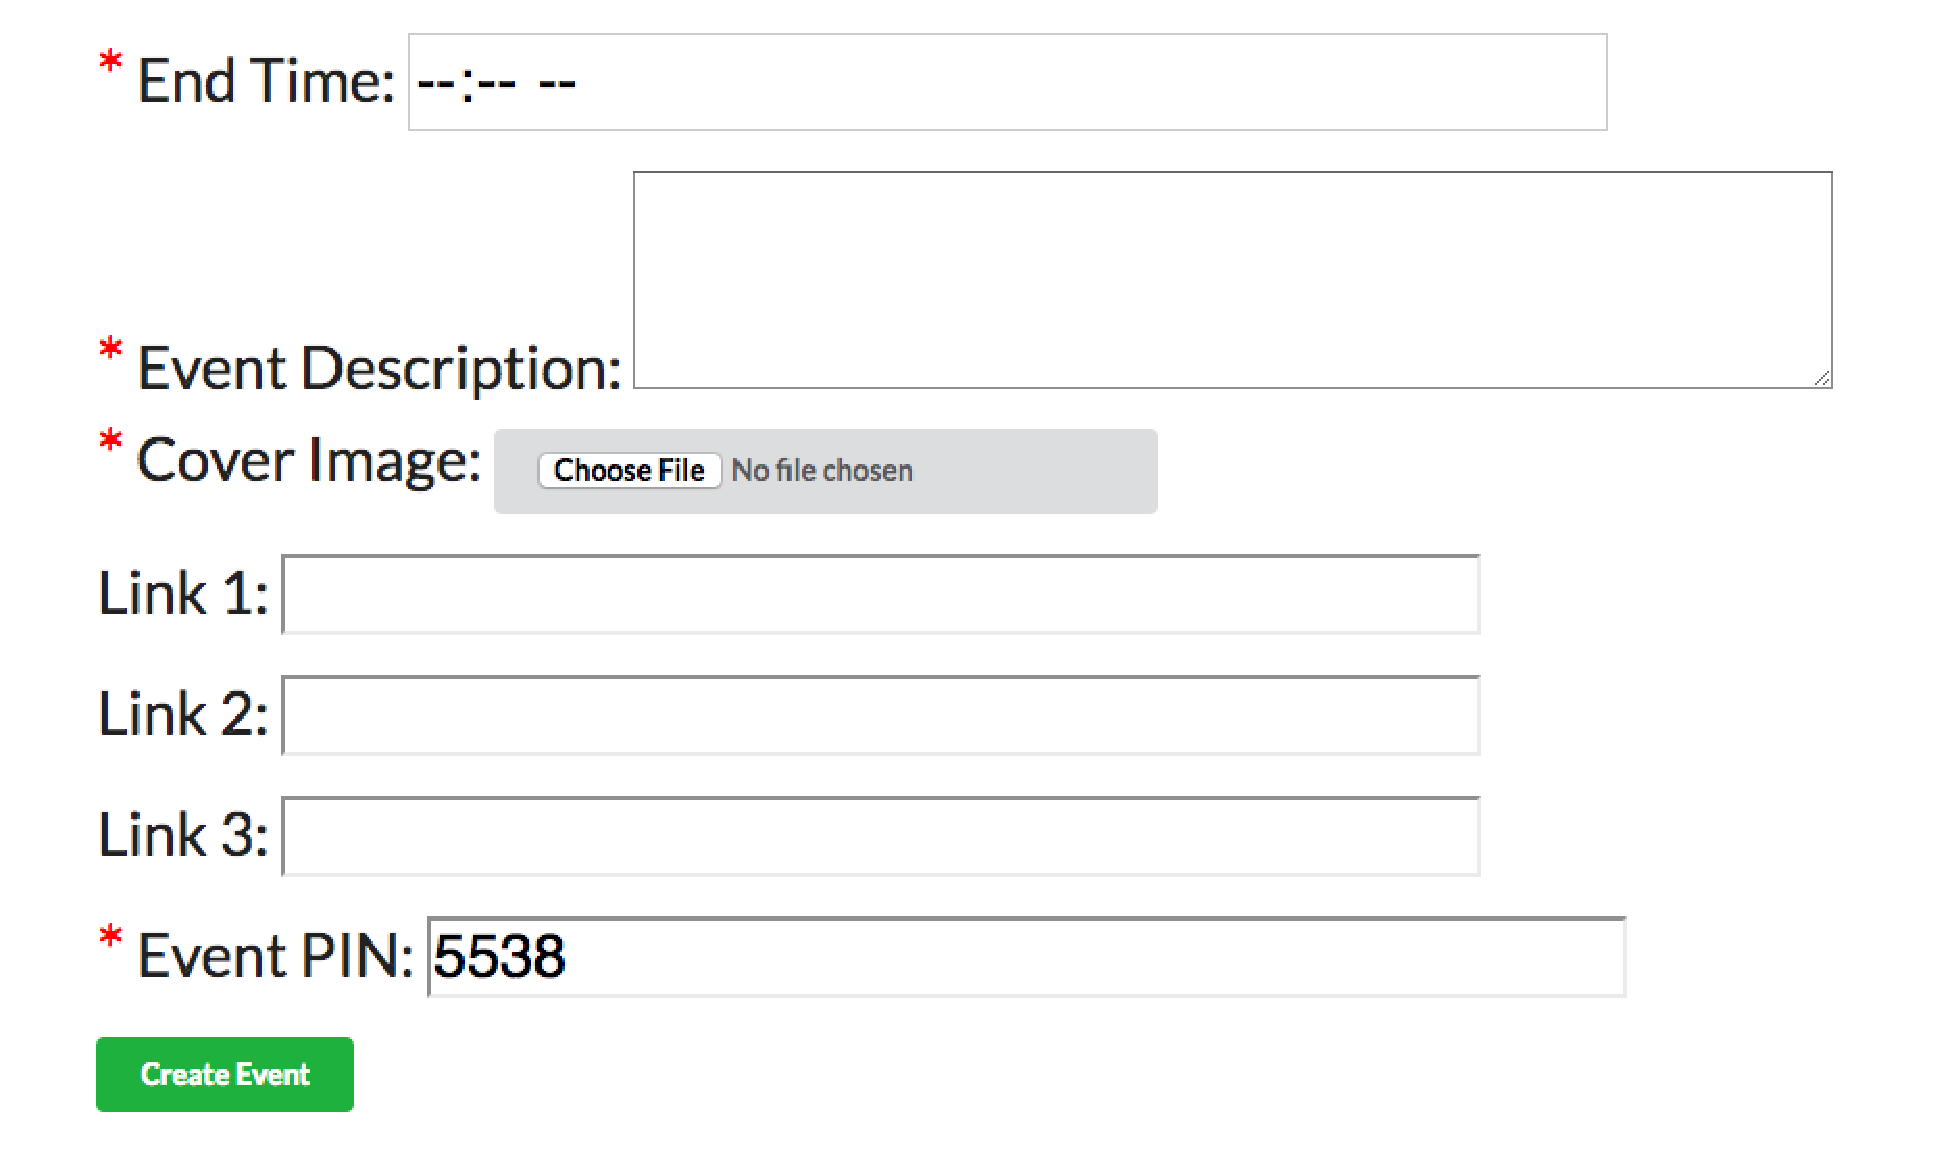
\includegraphics[height=5cm]{addcoverimage} \\
    Last term we had not implemented the functionality for our clients to add, modify or delete a photo from the event and resource pages. They now can successfully complete these actions as we have implemented the code into our web adminstration website. We did run into a couple of problems such as where and how to store the photos into our database. In order to work around this issue, we saved the path to the photo into our database and saved the photo itself in a seprate directory called images, which held subdirectories called "events," "resources" and "about."

  \subsection{Adding, Modifying, and Deleting Survey Questions}
    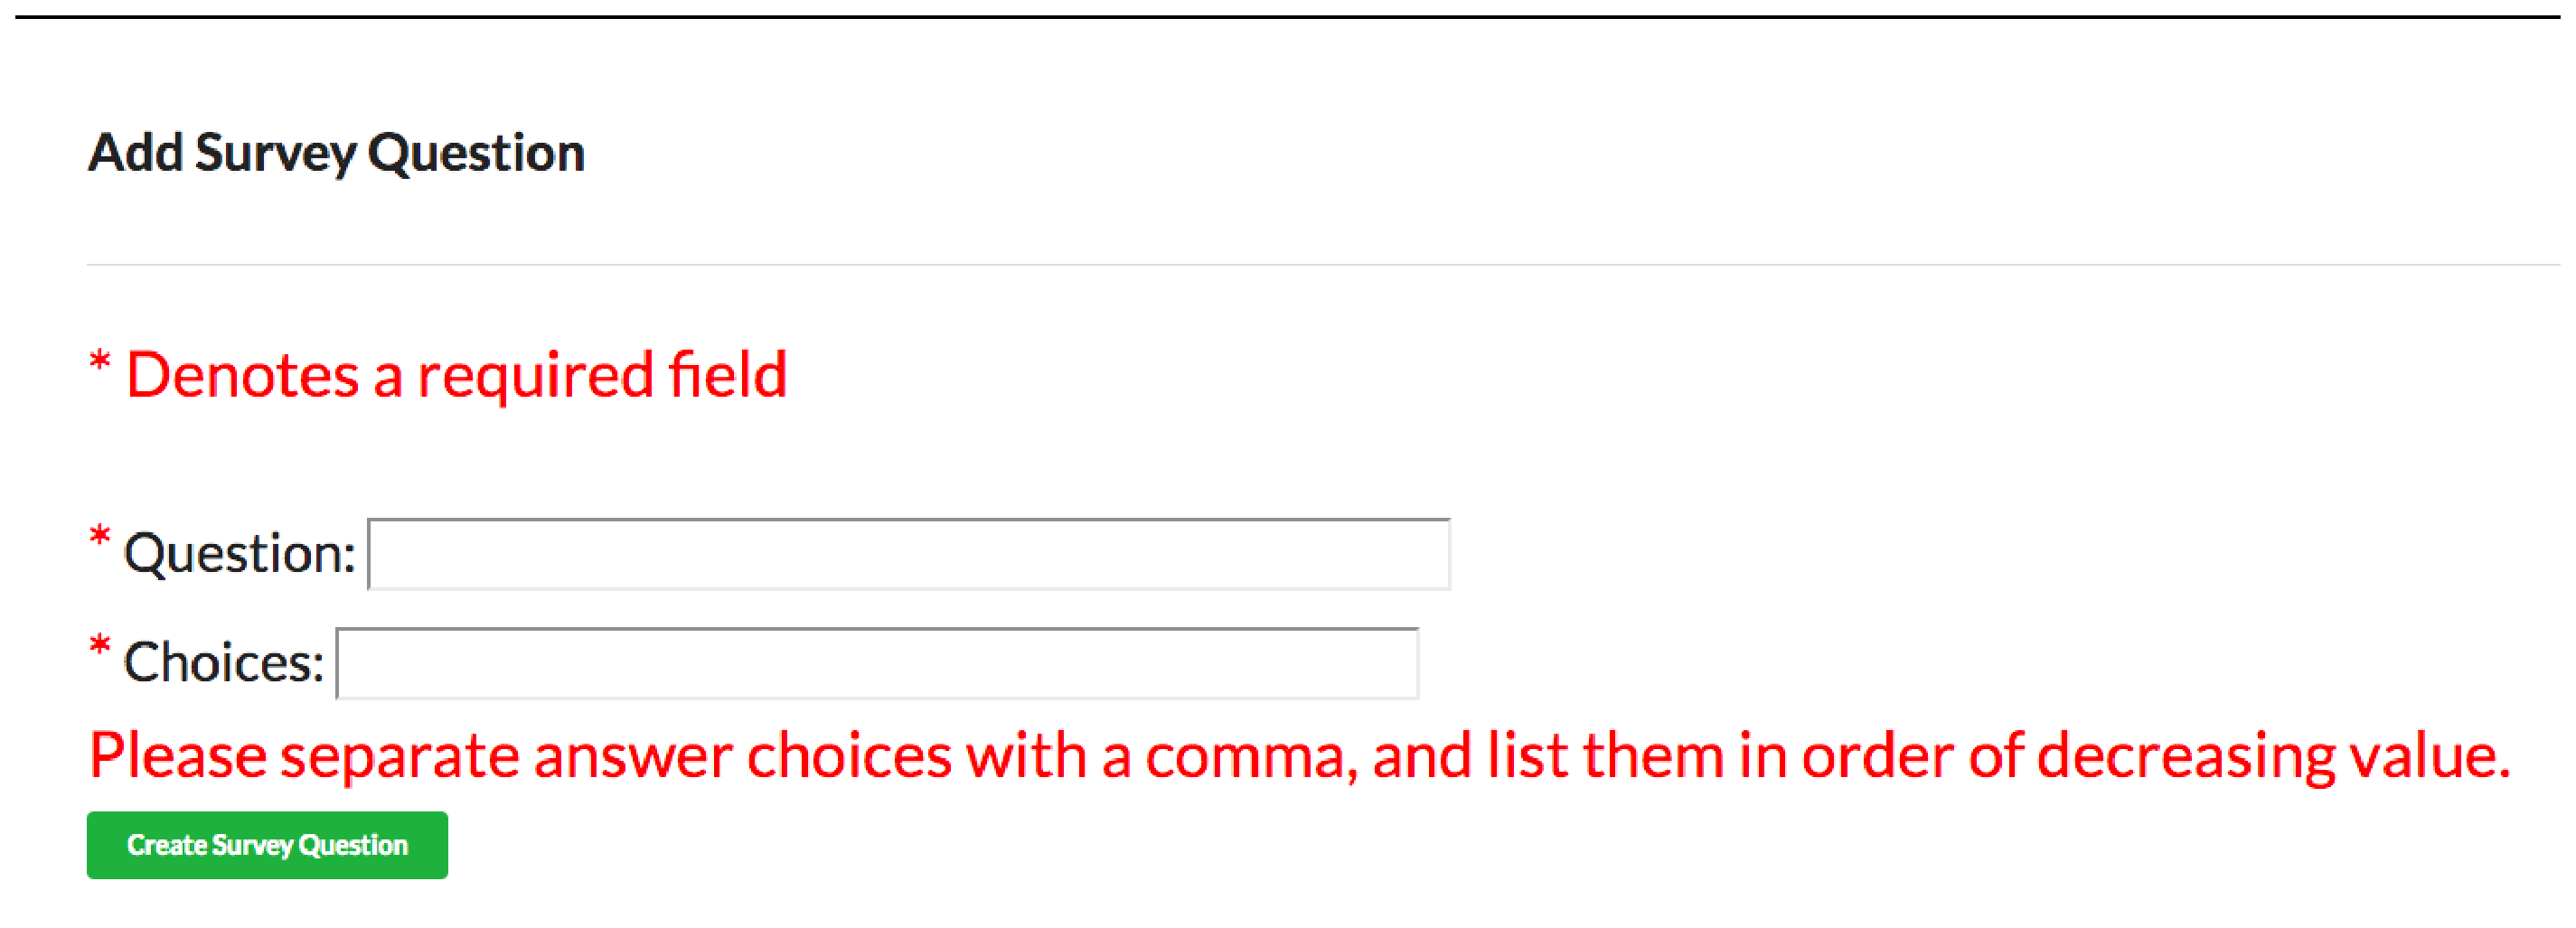
\includegraphics[height=4cm]{addsurveyquestion} \\
    \includegraphics[height=4cm]{managesurvey} \\
    Towards the end of Winter term, our client had asked us to implement a survery option for new users when first signing up. We implemented this feature at the beginning of this term, allowing our clients to successfully add, modify and delete survey questions through the website.

  \subsection{Form Validation}
    An error we had found at the beginning of the term was the failure of our form validation function when adding content through the website. The user would be able to miss a field and still be able to add content to the database. To patch this bug, we fixed some syntax errors in our form validation function, and it worked correctly. Below is an example of how our form validation works. Here, the code is validating the form for adding a new event.

    \begin{lstlisting}[style=javascript]
function validateForm() {
  var nameField = document.forms["eventForm"]["name"].value;
  var hostField = document.forms["eventForm"]["host"].value;
  var locationField = document.forms["eventForm"]["location"].value;
  var fullAddressField = document.forms["eventForm"]["fulladdress"].value;
  var setDateAndTimeField = document.forms["eventForm"]["setdateandtime"].value;
  var startDateField = document.forms["eventForm"]["startdate"].value;
  var startTimeField = document.forms["eventForm"]["starttime"].value;
  var endDateField = document.forms["eventForm"]["enddate"].value;
  var endTimeField = document.forms["eventForm"]["endtime"].value;
  var descriptionField = document.forms["eventForm"]["description"].value;
  var imageField = document.forms["eventForm"]["image"].value;
  var pinField = document.forms["eventForm"]["pin"].value;
  if (nameField == null || nameField == "" ||
      hostField == null || hostField == "" ||
      locationField == null || locationField == "" ||
      fullAddressField == null || fullAddressField == "" ||
      setDateAndTimeField == null || setDateAndTimeField == "" ||
      descriptionField == null || descriptionField == "" ||
      imageField == null || imageField == "" ||
      pinField == null || pinField == "") {
        alert("Please fill all required fields before submitting!");
        return false;
  }
  else {
    if (setDateAndTimeField == 1) {
      if (startDateField == null || startDateField == "" ||
      startTimeField == null || startTimeField == "" ||
      endDateField == null || endDateField == "" ||
      endTimeField == null || endTimeField == "") {
        alert("Please enter start and end dates and times!");
        return false;
      }
    }
    return true;
  }
}
    \end{lstlisting}

  \subsection{Prepared Statements}
    To protect our PHP scripts from SQL injection attacks, as well as to allow our client to use special characters like apostrophes in their text entries for new in-app entities, we have implemented PHP prepared statements in all of our scripts that properly format and sanitize values being input into the SQL query. An example of this is shown below. Here, we are using prepared statements to retrieve a particular user's completed events from the table of completed events.

    \begin{lstlisting}[style=php]
if ($_SERVER["REQUEST_METHOD"] == "POST") {
  $userid = $_POST['userid'];
  $stmt = $mysqli->prepare("SELECT E.* FROM ihc_events E, ihc_completed_events CE WHERE E.eventid=CE.eventid AND CE.userid=?");
  $stmt->bind_param('i', $userid);
  $stmt->execute();
  $res = $stmt->get_result();
  if ($res->num_rows > 0) {
    while ($event = $res->fetch_assoc()) {
      $data = json_encode($event);
      echo $data;
      echo "\\";
    }
  }
  $stmt->close();
}
    \end{lstlisting}

\section{Conclusion}
  At this point, we have fully completed the mobile application and administrative website to our clients full satisfaction. Our next steps will be to find a third-party service on which to host our database long-term, and to complete the demo version of the application and record a demo of the administrative website. Our goal is to have this completed at least a week before the Expo just in case we come across small problems or changes.

\end{document}
